\documentclass[12pt,a4paper]{article}

\usepackage[UTF8,zihao=-4]{ctex}
\usepackage[top=2.5cm,bottom=2.5cm,left=2.8cm,right=2.8cm]{geometry}
\usepackage{fontspec}
\setmainfont{Times New Roman}
\usepackage{setspace}
\setstretch{1.5}
\usepackage{amsmath,amssymb}
\usepackage{booktabs}
\usepackage{array}
\usepackage{makecell}
\usepackage{adjustbox}
\usepackage{graphicx}
\usepackage{subcaption}
\usepackage{float}
\usepackage{caption}
\usepackage{chngcntr}
\usepackage{enumitem}
\usepackage{fancyhdr}
\usepackage[hidelinks]{hyperref}

\setlength{\headheight}{15pt}
\pagestyle{fancy}
\fancyhf{}
\fancyhead[C]{\small 星点法测量透镜像差综合实验}
\fancyfoot[C]{\small\thepage}

\counterwithin{figure}{section}
\counterwithin{table}{section}
\renewcommand{\thefigure}{\thesection-\arabic{figure}}
\renewcommand{\thetable}{\thesection-\arabic{table}}
\captionsetup{font=small,labelsep=quad}
\graphicspath{{report_assets/}}
\setlist{nosep}

\begin{document}

\begin{titlepage}
  \centering
  \vspace*{2.2cm}
  {\heiti\zihao{2} 星点法测量透镜像差综合实验\par}
  \vspace{0.8cm}
  {\heiti\zihao{3} 实验报告\par}
  \vfill
  \begin{tabular}{rl}
    姓\quad 名： & \underline{\hspace{7cm}}\\[0.45cm]
    学\quad 号： & \underline{\hspace{7cm}}\\[0.45cm]
    班\quad 级： & \underline{\hspace{7cm}}\\[0.45cm]
    实验日期： & \underline{\hspace{7cm}}\\[0.45cm]
    指导教师： & \underline{\hspace{7cm}}
  \end{tabular}
  \vfill
\end{titlepage}

\section{实验目的}

\begin{enumerate}
  \item 理解透镜像差对点物成像质量的影响，认识星点像光强分布与光学系统像质之间的关系。
  \item 掌握用平行光管、环带光阑和 CMOS 相机测量透镜色差、球差和像散的基本方法。
  \item 通过蓝光、红光焦点位置差测量位置色差，通过像素坐标差换算倍率色差。
  \item 通过不同环带光阑的聚焦位置差和弥散斑大小分析球差，并通过透镜倾斜观察慧差和像散现象。
\end{enumerate}

\section{实验原理}

\subsection{星点法与点扩散}

理想光学系统应满足“点物成点像”。实际透镜受到衍射、材料色散、加工误差和几何像差影响后，一个很小的发光点经过系统成像时不会严格收缩为一点，而是在像面附近形成具有一定大小和形状的星点像。这个星点像可以看成光学系统对点物的响应，即点扩散函数。光斑越小、越对称，说明成像质量越好；若光斑变成圆环、拖尾或焦线，则说明系统存在相应的像差。

\subsection{色差测量原理}

透镜材料的折射率与波长有关。短波长光折射率较大，经过同一会聚透镜后焦距较短；长波长光折射率较小，焦距较长。因此蓝光和红光的最佳聚焦位置不同，形成位置色差。本实验先用蓝光 LED（451 nm）找到焦点并记录平移台读数 $X_1$，再换用红光 LED（690 nm）找到焦点并记录 $X_2$。位置色差为
\begin{equation}
  \Delta X = X_2-X_1 .
\end{equation}

在蓝光焦点位置换成红光后，红光在 CMOS 靶面上通常表现为弥散斑。若蓝光焦点参考像素坐标为 $b$，红光弥散斑边缘像素坐标为 $c$，CMOS 像素尺寸为 $2.9\,\mu\mathrm{m}$，倍率色差可按
\begin{equation}
  \Delta y = 2.9(c-b)\,\mu\mathrm{m}
\end{equation}
换算。式中正负号取决于软件像素坐标方向；讨论色差大小时通常取绝对值。

\subsection{球差测量原理}

球差是同一波长下不同孔径区域光线会聚位置不同造成的像差。对会聚透镜而言，近轴光线和边缘光线的焦点一般不完全重合。本实验在红光条件下先使用最小环带光阑寻找焦点，记录 $X_1$；再换大号环带光阑，在原焦面附近观察弥散光环，并重新调节 CMOS 相机寻找该环带对应焦点，记录 $X_2$。轴向球差的大小用两焦点轴向分离量表示：
\begin{equation}
  \left|\Delta X\right|=\left|X_2-X_1\right|.
\end{equation}
垂轴球差由弥散斑边缘与参考像素坐标差换算：
\begin{equation}
  \Delta h = 2.9(c-b)\,\mu\mathrm{m}.
\end{equation}

\subsection{慧差与像散}

慧差主要出现在轴外成像或透镜相对光轴倾斜时。此时不同孔径区域成像放大率不同，星点像会失去圆对称性，呈现类似彗星的亮头和拖尾。

像散是轴外光束在两个互相垂直的主截面内聚焦位置不同引起的。移动 CMOS 相机时，可以先看到一个方向的线状焦斑，再在另一轴向位置看到与其近似垂直的线状焦斑。两条焦线的轴向间隔反映像散大小：
\begin{equation}
  \left|\Delta X\right|=\left|X_2-X_1\right|.
\end{equation}

\section{实验仪器}

实验使用 LED 光源、平行光管、环带光阑、被测透镜、CMOS 相机、导轨与平移台等。色差测量使用蓝光 LED（451 nm）和红光 LED（690 nm）；单色像差测量主要使用红光 LED。被测透镜直径约为 40 mm，焦距约为 200 mm。CMOS 单个像素尺寸取 $2.9\,\mu\mathrm{m}$。环带光阑有不同孔径规格，色差测量保持同一小环带光阑，球差测量比较最小环带和大号环带，像散测量使用小环带并使透镜微倾。

\section{实验步骤}

\begin{enumerate}
  \item 调整 LED 光源、平行光管、光阑、被测透镜和 CMOS 相机的高度，使各元件中心尽量共轴。
  \item 测量色差时，先安装蓝光 LED 和小环带光阑，移动 CMOS 相机找到蓝光会聚点，记录平移台读数 $X_1$ 与像素参考坐标 $b$；随后换红光 LED，在原位置读取弥散斑边缘坐标 $c$，再移动相机找到红光焦点并记录 $X_2$。
  \item 测量球差时，使用红光 LED，先装最小环带光阑找到焦点并记录 $X_1$、$b$；再换大号环带光阑，记录弥散光环边缘坐标 $c$，继续移动相机找到大号环带焦点并记录 $X_2$。
  \item 观察慧差时，取下环带光阑，在找到星点焦点后将透镜旋转约 $20^\circ$，观察 CMOS 图像中星点像的非对称拖尾。
  \item 测量像散时，安装小环带光阑并使透镜分别倾斜约 $10^\circ$、$15^\circ$、$20^\circ$，沿导轨移动 CMOS 相机，分别记录两条互相垂直焦线出现时的平移台读数。
\end{enumerate}

\section{实验数据与处理}

\subsection{位置色差}

\begin{table}[H]
  \centering
  \caption{位置色差测量数据}
  \begin{adjustbox}{max width=\textwidth}
    \begin{tabular}{cccc}
      \toprule
      次数 & 蓝光焦点 $X_1$/mm & 红光焦点 $X_2$/mm & 位置色差 $\Delta X=X_2-X_1$/mm\\
      \midrule
      1 & 11.414 & 14.491 & 3.077\\
      2 & 11.598 & 14.585 & 2.987\\
      3 & 11.301 & 14.401 & 3.100\\
      \midrule
      平均值 & 11.438 & 14.492 & 3.055\\
      \bottomrule
    \end{tabular}
  \end{adjustbox}
\end{table}

三次测量得到的位置色差平均值为
\begin{equation}
  \overline{\Delta X}=3.055\,\mathrm{mm}.
\end{equation}
按三次重复测量估计，$\Delta X$ 的样本标准差约为 $0.060\,\mathrm{mm}$。

\subsection{倍率色差}

\begin{table}[H]
  \centering
  \caption{倍率色差测量数据}
  \begin{adjustbox}{max width=\textwidth}
    \begin{tabular}{ccccc}
      \toprule
      次数 & $b$/pixel & $c$/pixel & $c-b$/pixel & 倍率色差 $2.9(c-b)$/$\mu\mathrm{m}$\\
      \midrule
      1 & 397 & 390 & -7 & -20.3\\
      2 & 397 & 389 & -8 & -23.2\\
      3 & 395 & 390 & -5 & -14.5\\
      \midrule
      平均值 & 396.3 & 389.7 & -6.67 & -19.33\\
      \bottomrule
    \end{tabular}
  \end{adjustbox}
\end{table}

由数据记录可得，倍率色差的有符号平均值为 $-19.33\,\mu\mathrm{m}$。负号表示本次取点方向下红光弥散斑边缘坐标小于蓝光参考坐标；若只讨论色差大小，则为
\begin{equation}
  |\overline{\Delta y}|=19.33\,\mu\mathrm{m}.
\end{equation}

\subsection{红光球差}

\begin{table}[H]
  \centering
  \caption{红色光源轴向球差数据}
  \begin{adjustbox}{max width=\textwidth}
    \begin{tabular}{cccc}
      \toprule
      次数 & 最小环带焦点 $X_1$/mm & 大号环带焦点 $X_2$/mm & 轴向分离量 $|X_2-X_1|$/mm\\
      \midrule
      1 & 14.974 & 10.745 & 4.229\\
      2 & 14.845 & 10.378 & 4.467\\
      3 & 14.929 & 10.487 & 4.442\\
      \midrule
      平均值 & 14.916 & 10.537 & 4.379\\
      \bottomrule
    \end{tabular}
  \end{adjustbox}
\end{table}

由于记录单中大号环带焦点读数小于最小环带焦点读数，若严格按 $X_2-X_1$ 写有符号差值，其平均值为 $-4.379\,\mathrm{mm}$。本报告将球差作为轴向分离量讨论，因此取大小：
\begin{equation}
  |\overline{\Delta X}|=4.379\,\mathrm{mm}.
\end{equation}

\begin{table}[H]
  \centering
  \caption{红色光源垂轴球差数据}
  \begin{adjustbox}{max width=\textwidth}
    \begin{tabular}{ccccc}
      \toprule
      次数 & $b$/pixel & $c$/pixel & $c-b$/pixel & 垂轴球差 $2.9(c-b)$/$\mu\mathrm{m}$\\
      \midrule
      1 & 315 & 337 & 22 & 63.8\\
      2 & 315 & 333 & 18 & 52.2\\
      3 & 313 & 334 & 21 & 60.9\\
      \midrule
      平均值 & 314.3 & 334.7 & 20.33 & 58.97\\
      \bottomrule
    \end{tabular}
  \end{adjustbox}
\end{table}

由表中数据得到红光垂轴球差平均值为 $58.97\,\mu\mathrm{m}$。

\begin{figure}[H]
  \centering
  \begin{subfigure}{0.48\textwidth}
    \centering
    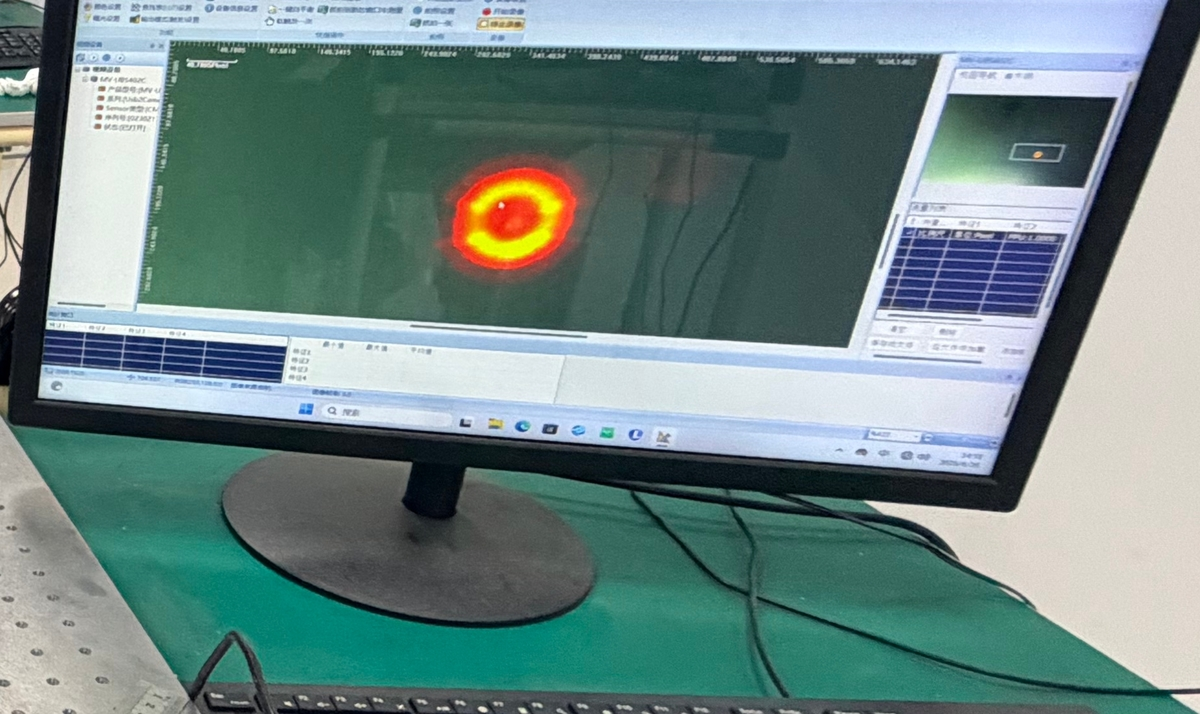
\includegraphics[width=\textwidth]{spherical_ring.jpg}
    \caption{大号环带下的弥散光环}
  \end{subfigure}
  \hfill
  \begin{subfigure}{0.48\textwidth}
    \centering
    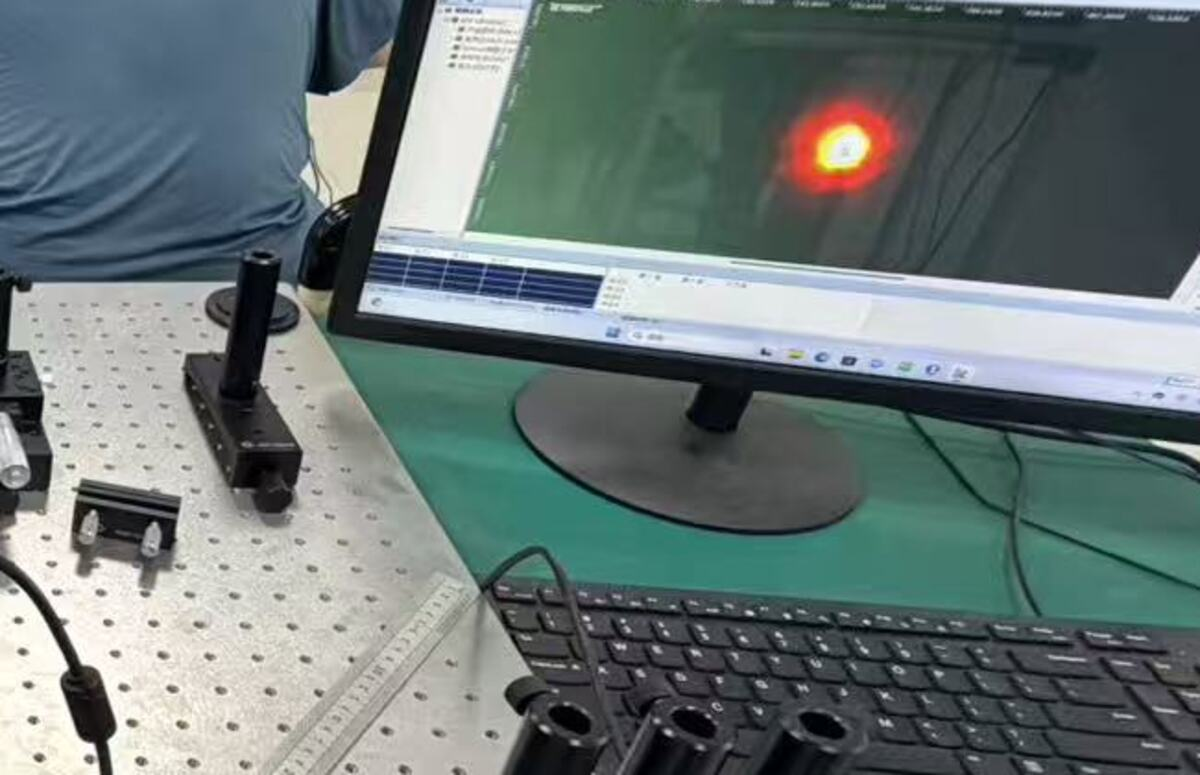
\includegraphics[width=\textwidth]{spherical_focus.jpg}
    \caption{重新调焦后的亮斑}
  \end{subfigure}
  \caption{红光球差测量中的典型星点像}
\end{figure}

\subsection{慧差观察}

在找到焦点后将透镜旋转约 $20^\circ$，CMOS 画面中星点像由近似圆斑变为明显的不对称拖尾图样。亮度集中在一端，另一侧呈扇形扩展，符合慧差的典型观察特征。

\begin{figure}[H]
  \centering
  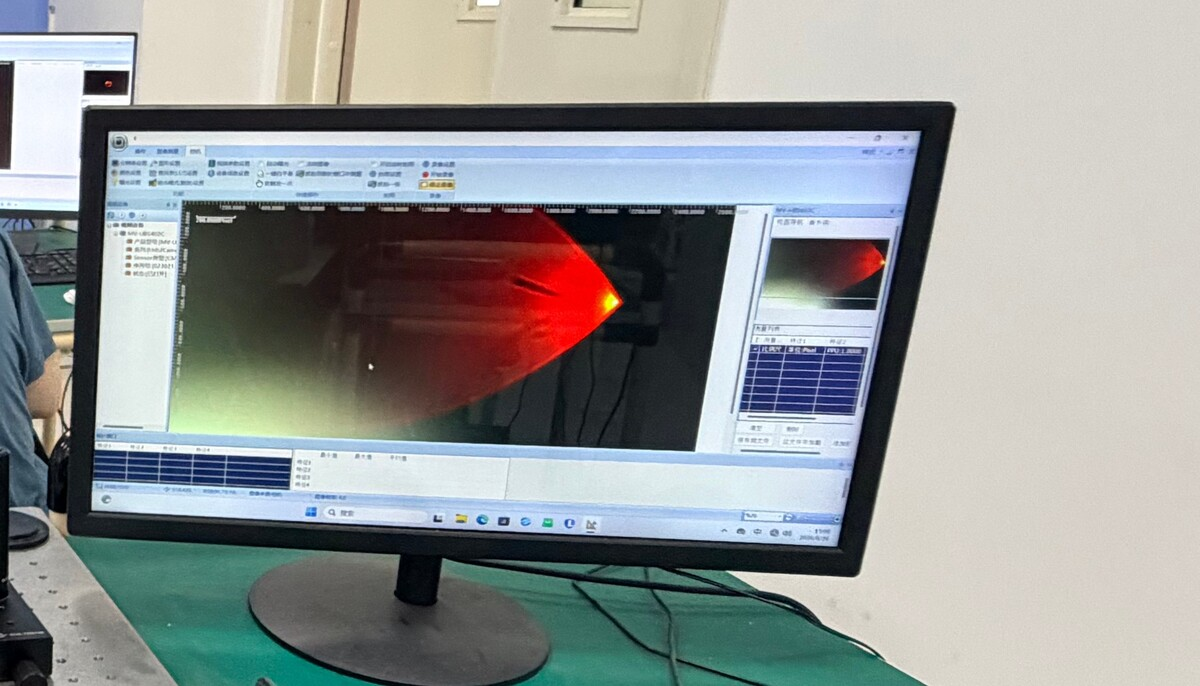
\includegraphics[width=0.82\textwidth]{coma_20deg.jpg}
  \caption{透镜旋转约 $20^\circ$ 时观察到的慧差图样}
\end{figure}

\subsection{像散}

\begin{table}[H]
  \centering
  \caption{像散测量数据}
  \begin{adjustbox}{max width=\textwidth}
    \begin{tabular}{ccccc}
      \toprule
      透镜倾角 & 次数 & $X_1$/mm & $X_2$/mm & 像散分离量 $|X_2-X_1|$/mm\\
      \midrule
      $20^\circ$ & 1 & 19.873 & 0.241 & 19.632\\
      $10^\circ$ & 2 & 4.955 & 0.382 & 4.573\\
      $15^\circ$ & 3 & 12.353 & 3.085 & 9.268\\
      \bottomrule
    \end{tabular}
  \end{adjustbox}
\end{table}

为便于比较，将不同倾角下的像散分离量按角度从小到大排列为
\[
  10^\circ:4.573\,\mathrm{mm},\quad
  15^\circ:9.268\,\mathrm{mm},\quad
  20^\circ:19.632\,\mathrm{mm}.
\]
可以看到透镜倾角增大时，两条焦线的轴向分离量明显增大。

\begin{figure}[H]
  \centering
  \begin{subfigure}{0.48\textwidth}
    \centering
    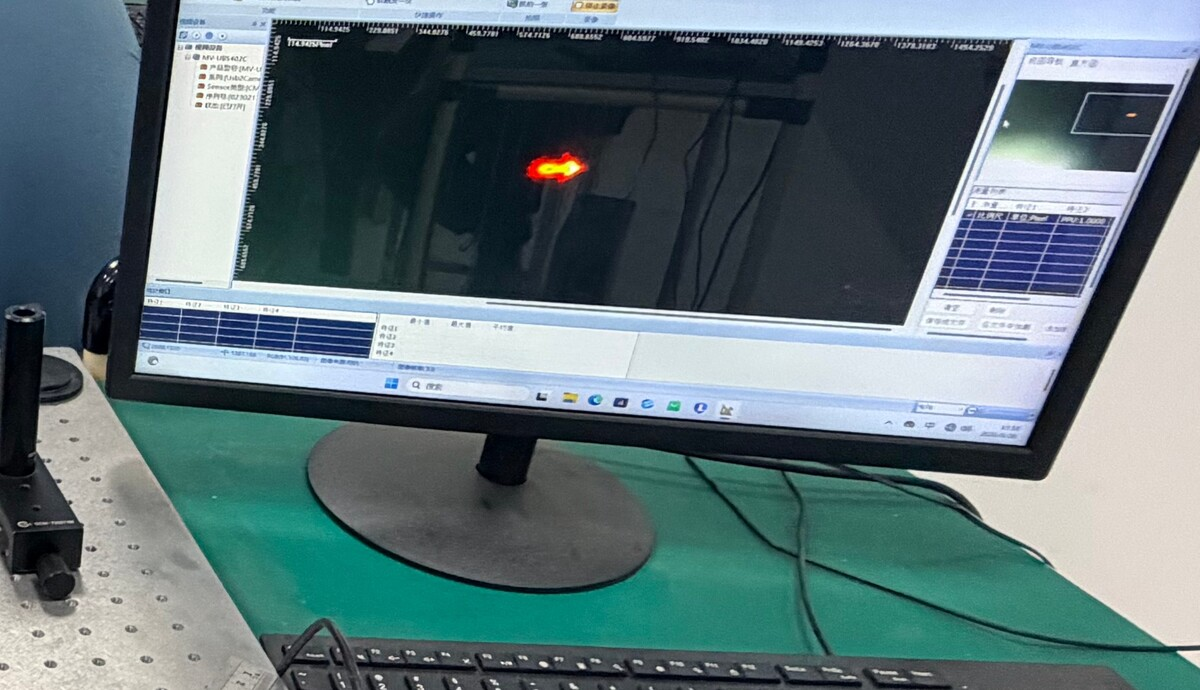
\includegraphics[width=\textwidth]{astig_horizontal.jpg}
    \caption{水平焦线}
  \end{subfigure}
  \hfill
  \begin{subfigure}{0.48\textwidth}
    \centering
    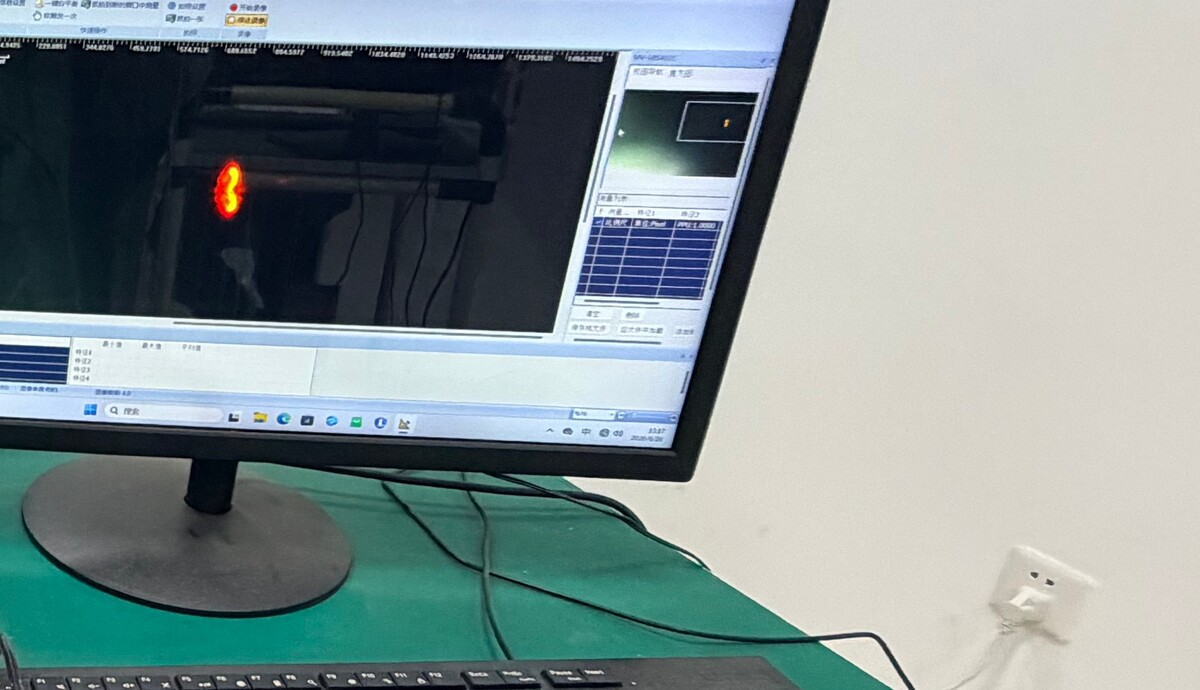
\includegraphics[width=\textwidth]{astig_vertical.jpg}
    \caption{竖直焦线}
  \end{subfigure}
  \caption{透镜倾斜约 $10^\circ$ 时观察到的像散焦线}
\end{figure}

\section{实验结果与分析}

\subsection{色差结果分析}

蓝光焦点平均读数为 $11.438\,\mathrm{mm}$，红光焦点平均读数为 $14.492\,\mathrm{mm}$，红光焦点读数更大，二者相差 $3.055\,\mathrm{mm}$。这说明在本实验的读数方向上，红光的最佳成像位置比蓝光更远，符合普通玻璃透镜中红光折射率较小、焦距较长的规律。

倍率色差的有符号平均值为 $-19.33\,\mu\mathrm{m}$。由于像素坐标方向由 CMOS 软件定义，符号主要反映所选边缘方向；从大小看，红光弥散斑相对蓝光参考坐标存在约 $19.33\,\mu\mathrm{m}$ 的横向偏移，说明不同波长光不仅焦点轴向位置不同，在同一像面处的像高也存在差异。

\subsection{球差结果分析}

红光球差测量中，最小环带焦点平均读数为 $14.916\,\mathrm{mm}$，大号环带焦点平均读数为 $10.537\,\mathrm{mm}$，轴向分离量为 $4.379\,\mathrm{mm}$。实验现象中，在一个环带的焦面处更换另一环带后出现明显弥散环，继续移动相机后又能重新形成较集中的亮斑，说明不同孔径区域的光线确实不在同一轴向位置会聚。

垂轴球差平均值为 $58.97\,\mu\mathrm{m}$，明显大于倍率色差的横向量级。这说明在本实验条件下，不同孔径区域引起的横向弥散比红蓝光倍率差异更显著。由于大号环带主要选取较远离光轴的光线，该结果反映了边缘光线与近轴光线会聚位置不一致所造成的像质下降。

\subsection{慧差与像散结果分析}

透镜旋转约 $20^\circ$ 后，星点像出现明显非对称拖尾，亮头和尾部不再关于光轴对称。这与慧差的形成机制一致：透镜倾斜相当于引入轴外光束，不同孔径区域的成像放大率和会聚位置不同，导致点像被拉成类似彗星的形状。

像散测量显示，倾角约 $10^\circ$、$15^\circ$、$20^\circ$ 时的焦线分离量分别为 $4.573\,\mathrm{mm}$、$9.268\,\mathrm{mm}$、$19.632\,\mathrm{mm}$。随着倾角增大，子午方向和弧矢方向的聚焦差异增大，像散更明显。该变化趋势与轴外像差随视场角或倾角增大而增强的理论判断一致。

\section{误差分析}

\begin{enumerate}
  \item \textbf{焦点判定误差。} 星点像在焦点附近并不是突然变为最小，而是在一段轴向范围内缓慢变化。若每次判断“最亮、最小”标准不完全一致，会直接影响 $X_1$、$X_2$ 读数。
  \item \textbf{平移台读数与回程间隙。} 若寻找焦点时移动方向不一致，丝杆或平移台可能存在回程间隙，使同一实际位置对应不同读数。较好的做法是每次都从同一方向逼近焦点。
  \item \textbf{像素坐标点击误差。} 弥散斑边缘亮度渐变，边界不锐利；曝光过强时边缘会扩大，曝光过弱时边缘难以判断，都会影响 $b$、$c$ 的读取。
  \item \textbf{光路共轴误差。} 光源、平行光管、光阑、透镜和 CMOS 相机若不同轴，会把装调偏心引起的光斑偏移混入色差、球差和像散测量。
  \item \textbf{换光源和换光阑引入的扰动。} 色差测量需要更换蓝光和红光 LED，球差测量需要更换环带光阑；若更换后高度或中心位置发生改变，会使测量结果包含机械位置误差。
  \item \textbf{倾角估计误差。} 慧差和像散观察中透镜倾角主要由机械刻度或人工调节估计，实际角度可能与记录角度存在偏差，因此像散随倾角变化的结论更适合做定性和半定量分析。
\end{enumerate}

\section{实验结论}

本实验利用星点法测量并观察了透镜的典型像差。色差测量得到蓝光与红光焦点的轴向位置差为 $3.055\,\mathrm{mm}$，红光焦点相对蓝光焦点更远；倍率色差的大小约为 $19.33\,\mu\mathrm{m}$。红光球差测量得到不同环带光线的轴向焦点分离量为 $4.379\,\mathrm{mm}$，垂轴球差约为 $58.97\,\mu\mathrm{m}$，说明孔径不同会显著改变星点像的会聚位置和弥散程度。

在透镜倾斜条件下，实验观察到明显的慧差拖尾和像散焦线。像散测量结果表明，当倾角由约 $10^\circ$ 增大到 $20^\circ$ 时，焦线分离量由 $4.573\,\mathrm{mm}$ 增大到 $19.632\,\mathrm{mm}$，说明轴外或倾斜条件会显著降低点成像质量。整体来看，星点法能够通过直观的光斑形状和可测的轴向、横向数据，有效反映透镜的色差、球差、慧差和像散。

\section*{参考文献}
\addcontentsline{toc}{section}{参考文献}

\begin{thebibliography}{9}
  \bibitem{zhu2004} 朱瑶. 光学系统的星点检验方法[J]. 红外, 2004(9): 31--37.
  \bibitem{yu2011} 郁道银, 谈恒英. 工程光学[M]. 北京: 机械工业出版社, 2011.
  \bibitem{yao2002} 姚启钧, 华东师范大学光学教材编写组改编. 光学教程[M]. 第3版. 北京: 高等教育出版社, 2002.
\end{thebibliography}

\end{document}
